\subsection{Distancia euclidiana}
En matemáticas, la distancia euclidiana o euclídea, es la distancia ordinaria entre dos puntos de un espacio euclídeo, la cual se deduce a partir del teorema de Pitágoras. 

$$ d_{E}(P_{1},P_{2})={\sqrt {(x_{2}-x_{1})^{2}+(y_{2}-y_{1})^{2}}} $$

En general, la distancia euclidiana entre los puntos $P=(p_{1},p_{2},\dots ,p_{n})$ y $Q=(q_{1},q_{2},\dots ,q_{n})$, del espacio euclídeo n-dimensional, se define como: 

$$ d_{E}(P,Q)={\sqrt {(p_{1}-q_{1})^{2}+(p_{2}-q_{2})^{2}+\cdots +(p_{n}-q_{n})^{2}}}={\sqrt {\sum _{i=1}^{n}(p_{i}-q_{i})^{2}}} $$

\subsection{Polígono}

Un polígono es una figura plana que está delimitada por un camino cerrado (camino que comienza y termina en el mismo vértice) compuesto por una secuencia finita de segmentos de línea recta. estos segmentos se llaman aristas o lados. El punto donde se unen dos aristas es el vértice o esquina del polígono. Dentro de los elementos que distiguen a un polígono podemos citar:

% TODO: \usepackage{graphicx} required
\begin{figure}[h!]
	\centering
	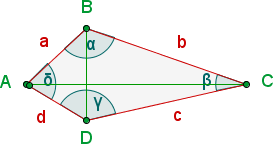
\includegraphics[width=0.35\linewidth]{img/elementos-de-un-poligono}
	\caption{Ejemplo de un polígono}
	\label{fig:elementos-de-un-poligono}
\end{figure}


\begin{enumerate}
	\item \textbf{Lados:} Los lados de un polígono son los segmentos que lo limitan.
	\item \textbf{Vértices:} Los vértices son los puntos donde concurren dos lados. En la figura de arriba, los vértices son los puntos A, B, C, y D.
	\item \textbf{Ángulos interiores:} Los ángulos interiores son determinados por dos lados consecutivos. En la figura de arriba, tenemos los ángulos $\alpha$, $\beta$, $\bar{o}$, y $Y$. Para sumar los ángulos interiores de un polígono,si $n$ es el número de lados, tenemos la siguiente fórmula: Suma de los ángulos interiores de un polígono $= (n - 2) \cdot 180°$
	\item \textbf{Diagonales:} Las diagonales son los segmentos que determinan dos vértices no consecutivos. En la figura precedente, tenemos dos diagonales, el segmento que uno los vértices A y C, y el segmento que une los vértices B y D. Para averiguar el número de diagonales de un polígono, si n es el número de lados, podemos usar la siguiente fórmula: Número de diagonales de un polígono $= n \cdot (n - 3) \div 2$
\end{enumerate}